%!TEX root = Bericht.tex
\graphicspath{{graphics/HMI/}{graphics/control_modes/}}
\chapter{The different Control Modes}
\label{cha:DifferentControlModes}

\textbf{\textit{About the need of different modes, the requirements of image capturing and an overview of the realized modes}} \\

As mentioned in section \ref{sec:system overview}, one of \textsc{Skye}'s unique properties are the decoupled 6DOF in space. This means, the system has the possibility to turn around an arbitrary axis while moving in any direction. This ability has to be used to fulfill the operation tasks in an optimal way. An intuitive handling for the pilot has to be granted in any way. \\ 
The first approach is to provide a manual control mode that allows the pilot to directly control the 6DOF. A detailed description will be given in section \ref{sec:manualControlModes}. \\ 
In contrast to the unrestricted control possibilities for manual control, a more autonomous control would allow the pilot to focus on a specific motion, e.g. the orientation of the camera. Therefore, a part of the 6DOF motion of \textit{Skye} will be automated\footnote{The prototype designed for this project does not include any environment detections. Therefore, autonomous control with obstacle detection will not yet be possible.}. In section \ref{sec:automaticControlModes} this is described in more detail. Furthermore, a basic \textit{test phase} control mode lets the operator directly access the 8 actuators individually. Table \ref{tab:control_modes} gives an overview of the control modes. Those actual realization is presented in chapter \ref{cha:findHardSoftSolution}.

\begin{table}[h]		% [H] indicates that the table should be right here.
	\begin{tabular}{c c c c c} %{p{0.16\textwidth}p{0.16\textwidth}p{0.16\textwidth}p{0.16\textwidth}p{0.16\textwidth}}	% add p{size_of_column} for every new column you'd like to have. If you put a | between the p then there is a vertical line between the columns. 
	Test Phase 		& Direct Control 	& Assisted Control 	& Half Automatic	& Full Automatic  \\
	\toprule[1.25pt]				%define the line thickness of the top rule
	Thrust 1		& Thrust $x$	& Velocity $x$	& Velocity	& Velocity	\\
	Thrust 2		& Thrust $y$	& \textit{Velocity $y$}	& Rotation $x$	& Rotation $x$\\
	Thrust 3		& Thrust $z$	& \textit{Velocity $z$}	& Rotation $y$	& Waypoints	\\
	Thrust 4		& Moment $x$	& Rotation $x$	& Rotation $z$	&	Camera target\\
	Direction 1		& Moment $y$	& Rotation $y$	& Waypoints	&	\\
	Direction 2		& Moment $z$	& Rotation $z$	&		&	\\
	Direction 3		& 		& 		&		&	\\
	Direction 4		& 		& 		&		&	\\

	\bottomrule[1.25pt]
	\end{tabular} 
	\caption[The different control modes]{With the control modes, different inputs are given to the controller. The inputs in \textit{italic} are not available for \textit{Assisted RC  Control}.}
	\label{tab:control_modes}
\end{table}

\section{Manual Control Modes}
\label{sec:manualControlModes}
\textit{Test Phase, Direct Control and Assisted Control}
\subsubsection{Test Phase} 
As the prototype \textsc{Skye} was built in parallel to this thesis, the overall functionality of the system had to be checked piecewise. The \textit{test phase} control mode was therefore designed to test the propulsion's behaviour. The number of revolutions as well as the reference orientation of each of the four actuation units can be set individually\footnote{In \cite{schaffnervu} referred to as input for the \textit{Thrust Section} and \textit{Positioning Section} respectively.}.

\begin{figure}[H] % [H] steht dafür, dass das Bild genau hier im Text sein soll.
	\begin{center}
		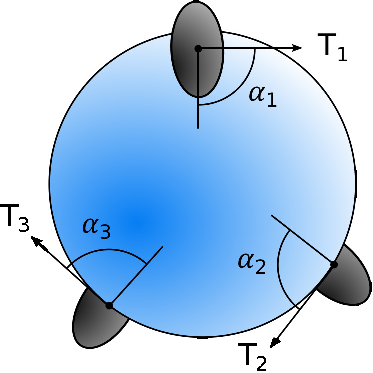
\includegraphics[width=0.3\textwidth]{TPC.pdf}
		\caption[Test Phase]{Test Phase}  
		\label{fig:test_phase}		
	\end{center}
\end{figure}


\subsubsection{Direct Control} 
A second control mode that mainly intends to verify the system's properties is the \textit{direct control} mode where the operator sets the desired force and moment vectors. This 6DOF control therefore needs the transformation of the forces and moments to the 8 actuators\footnote{See \cite{schaffnervu} for details about the optimization criteria for the motor allocation.} only. No information about the system's properties and states are needed. The pilot's input is interpreted as the force and moment components in body fixed coordinates. As the camera system (the eye of \textsc{Skye}) enables best to recognize \textsc{Skye}'s attitude, the coordinate frame was aligned to the camera's orientation. This is illustrated in figure \ref{fig:direct_control}, where $\{e_x^C, e_y^C, e_z^C\}$ represents the camera orientated frame ($e_x^C$ collinear with the camera axis, $e_y^C$ pointing to the right, $e_z^C$  pointing downwards) and $\{F_x^C, F_y^C, F_z^C, M_x^C, M_y^C, M_z^C\}$ the user input.

%\begin{figure}[H] % [H] steht dafür, dass das Bild genau hier im Text sein soll.
%	\begin{center}
%		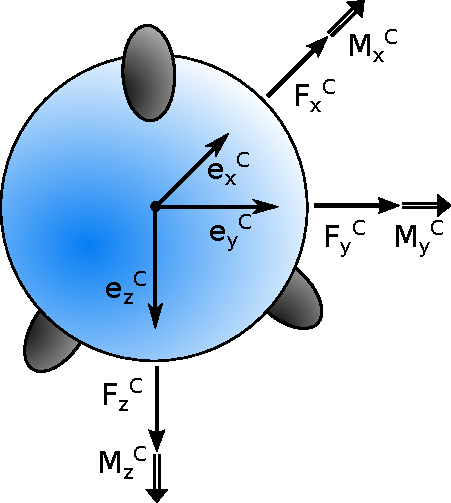
\includegraphics[width=0.37\textwidth]{DC.pdf}
%		\caption[Direct control]{Direct Control}  
%		\label{fig:direct_control}
%	\end{center}
%\end{figure}

\begin{figure}[H]		
	\small{
		\begin{center}
			\parbox{0.36\textwidth}{\centering 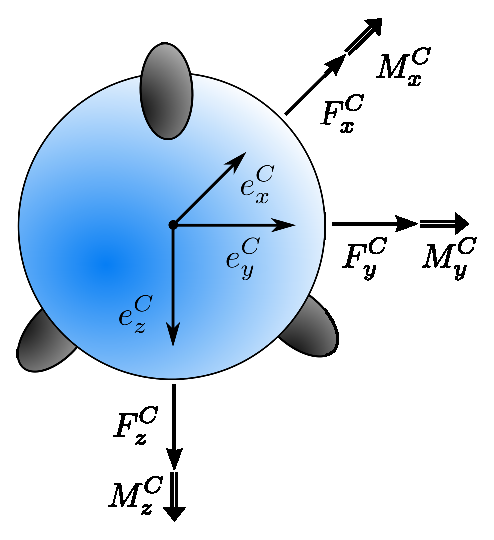
\includegraphics[width=0.36\textwidth]{DC}
			 Direct Control}
			\hspace{0.1\textwidth}			
			\parbox{0.36\textwidth}{\centering 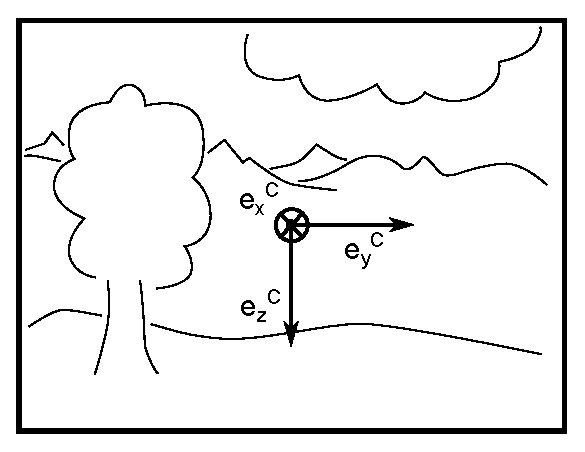
\includegraphics[width=0.36\textwidth]{CameraFrame}
			Camera Frame}
	\caption[Assisted Control]{Direct Control (left) and the orientation of the camera frame in relation to the camera's field of view (right).}
		\label{fig:direct_control}
		\end{center}
	}			
	\vspace{4.5mm}
\end{figure}


\subsubsection{Assisted Control} 
The \textit{direct control} mode demands well trained skills to properly navigate \textit{Skye}. This is especially due to the low damped rotations \cite{weichart} and the symmetrical appearance of the system. To cope with the low damped rotations, a stabilizing attitude controller is needed. In order to better deal with the symmetrical appearance, the translational inputs can be interpreted in a earth fixed coordinate frame. By using a proper state estimation, the pilot's commands can directly be interpreted as velocities and angular velocities respectively\footnote{See \cite{meiermueri} for the state estimation and controller design.}. This is actually realized in the \textit{assisted control} mode. Figure \ref{fig:assisted_control} illustrates the user's input $\{v_x^I, v_y^I, v_z^I, \omega_x^C, \omega_y^C, \omega_z^C\}$. \\
If a user interface for less than 6DOF is used, e.g. a remote controller\footnote{A remote controller (RC) was implemented as redundant control link, see section \ref{sub:hardware} or \cite{burri}.} which has only 4DOF, the user input is restricted to $\{v_x^C, \omega_x^C, \omega_y^C, \omega_z^C\}$ which is similar to helicopter or airplane control.

\begin{figure}[H]		
	\small{
		\begin{center}
			\parbox{0.36\textwidth}{\centering 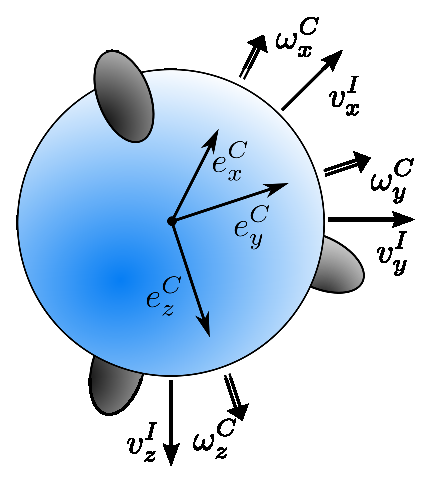
\includegraphics[width=0.36\textwidth]{AC}
			 Assisted Control}
			\hspace{0.1\textwidth}			
			\parbox{0.36\textwidth}{\centering 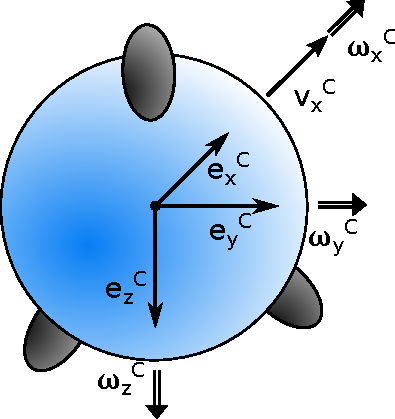
\includegraphics[width=0.36\textwidth]{RC}
			Assisted RC Control}
	\caption[Assisted Control]{Assisted Control with controlling six (left) and four (right) stabilized degrees of freedom.}
		\label{fig:assisted_control}
		\end{center}
	}			
	\vspace{4.5mm}
\end{figure}

\section{Automatic Control Modes}
\label{sec:automaticControlModes}
\textit{Half Automatic Control and Full Automatic Control}

\subsubsection{Half Automatic Control}
When scanning an object for 3d reconstruction, it is often clear in advance where the pictures should be taken from. Therefore, a waypoint based controlling would be desirable. The \textit{half automatic control} mode allows to define a set of waypoints\footnote{In \cite{biagiotti} the waypoints are called \textit{via-points}.} $\{{\bf q}_0, {\bf q}_1, \cdots, {\bf q}_n\}$ for the system's position. The rotational degrees of freedom $\{\omega_x^C, \omega_y^C, \omega_z^C\}$ remain manually controllable. This allows to adjust the camera's orientation while automatically following the given path. For convenient use, it is important that the user can reduce the translational velocity on the path for instance if an additional view at the current position is demanded.

\begin{figure}[H] % [H] steht dafür, dass das Bild genau hier im Text sein soll.
	\begin{center}
		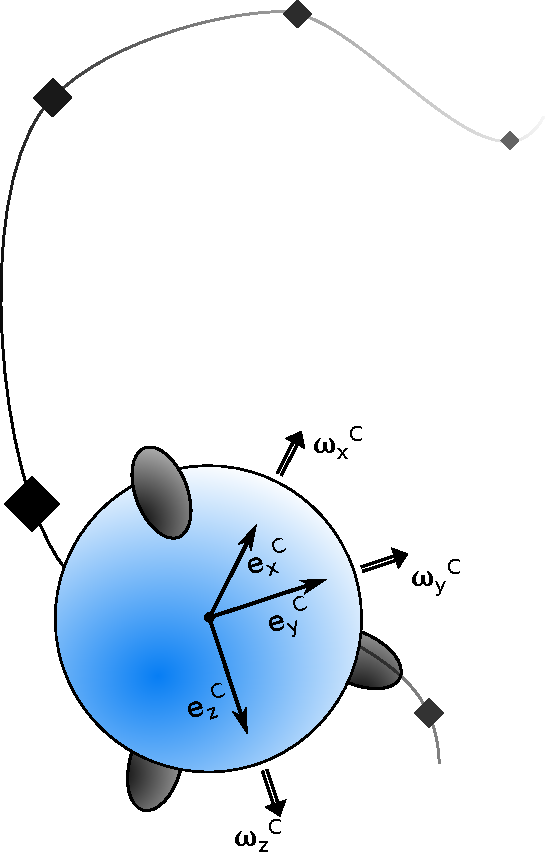
\includegraphics[width=0.4\textwidth]{HAC.pdf}
		\caption[Half automatic control]{Half Automatic Control}  
		\label{fig:half_automatic_control}		
	\end{center}
\end{figure}

\subsubsection{Full Automatic Control}
An even more advanced control mode would also automatically adjust the system's orientation. Therefore, also the camera target position has to be indicated. For this Bachelor's thesis, only a solution considering a fix target point has been elaborated. This could easily be extended to multiple targets point similar to the waypoints. \\ As it can be seen in figure \ref{fig:full_automatic_control}, even with this method the orientation around the camera axis $e_x^C$ is not defined explicitly. Therefore, $\omega_x^C$ would remain as a manual user input. Indeed, for capturing images it is convenient to adjust the orientation to keep the horizon aligned.


\begin{figure}[H] % [H] steht dafür, dass das Bild genau hier im Text sein soll.
	\begin{center}
		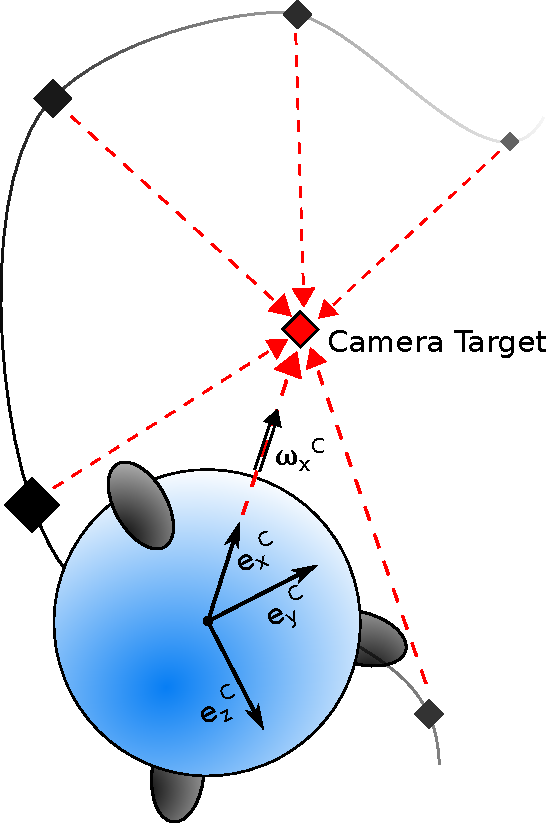
\includegraphics[width=0.4\textwidth]{FAComega.pdf}
		\caption[Full automatic control]{Full Automatic Control.}  
		\label{fig:full_automatic_control}		
	\end{center}
\end{figure}